\newpage
\chapter{Especificações de máquina}

Neste capítulo, são apresentados os materiais escolhidos e as especificações da máquina, como por exemplo o volume de trabalho, a precisão e a velocidade de usinagem, parâmetros essenciais para a compreensão do funcionamento de um torno.

\section{Materiais}

Dentre os materiais disponíveis, esse grupo selecionou os seguintes: 
\begin{itemize}
    \item Inversor CFM 500
    \item Correia sincronizadora Optibelt ZR 345L
    \item Polia 26 L 075 
    \item Polia 48 L 075
    \item Mesa deslizante 3 (430 mm) e 4 (280 mm)
    \item 2x Motor KTC HT-23-400
    \item 2x Acoplamento fole (tipo 3)
\end{itemize}
%%%%%%%%%%%%%%%%%%%%%%%%%%%%%%%%%%%%%%%%%%%%%%%%%%%%%%%%%%%%%%%

\section{Eixo árvore}
O eixo árvore especificado para a máquina é composto por uma placa de três castanhas para fixação da peça, perfil tubular de aço com seção quadrada de 100 mm de lado e 3,18 mm de parede, rolamentos radiais de esferas, polia para correia sincronizadora e encoder óptico.

Seguem as imagens que especificam o funcionamento do encoder óptico e também o rolamento de esferas:

\begin{figure}[h!]
    \centering
    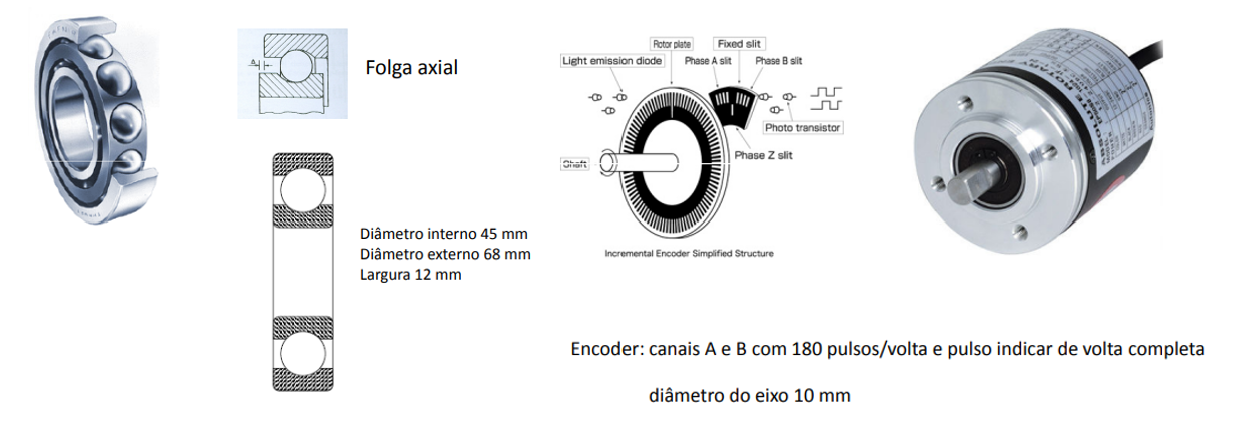
\includegraphics[width=\linewidth]{images/rolamentos.png}
    \label{fig:enter-label}
\end{figure}

\subsection{Potência}

De acordo com as especificações iniciais do motor CA que transmitirá movimento à máquina por meio da transmissão por correia, a sua potência fornecida é de 0,5 HP, dada uma tensão de 220V e uma rotação de 1720rpm.

As potências fornecidas pelo motor de passo, no entanto, variam de modelo para modelo. Considerando o motor KTC-HT23-401, temos diferentes valores a depender da operação (torque transmitido e respectiva velocidade angular). 

O motor KTC-HT23-400 possui uma curva de torque dada o valor do par revoluções por segundo e torque que transmite a maior potência para o sistema é um torque de 0,67Nm a uma rotação de 15 revoluções por segundo, que gera uma potência de 0,08468 HP.

\begin{figure}[h!]
    \centering
    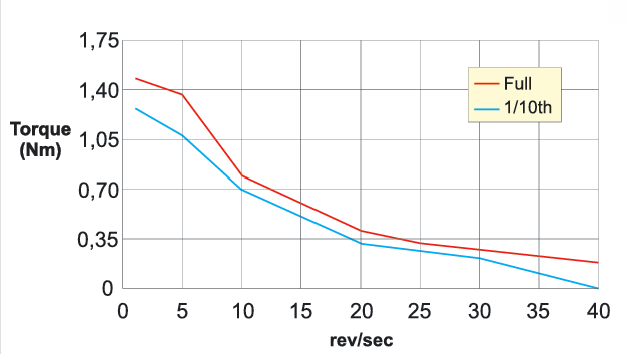
\includegraphics[width=0.8\linewidth]{images/torque.png}
    \caption{Curva de torque do motor de passo KTC-HT23-400 \cite{kalatec2020catalogo}.}
    \label{fig:enter-label}
\end{figure}

\subsection{Rotação}

Levando em consideração a tabela e sabendo que o inversor a ser utilizado armazena até 8 velocidades, podemos escolhê-las de acordo com a ferramenta, que será de aço rápido, e o material usinado, que será de material mole (para as presentes especificações utiliza-se o Nylon). Deve-se levar também em conta que a placa de castanhas possui limitação de rotação de 900 RPM. 

Considerando um peça de nylon de diâmetro máximo 100mm a rotação do eixo necessária, de acordo com a equação 21, na seção 13.1, para as operações de usinagem é 955 RPM. Esse valor aumentará de forma inversamente proporcional ao diâmetro a peça. 

As demais 8 rotações serão ainda escolhidas para cada processo (acabamento, desbaste e rosqueamento) e diâmetro disponível da peça. Em seguida, elas serão programadas no inversor para a usinagem das peças.  

%%%%%%%%%%%%%%%%%%%%%%%%%%%%%%%%%%%%%%%%%%%%%%%%%%%%%%%%%%%%%%%
\section{Especificações Elétricas}

Para as especificações elétricas foram analisados dados elétricos dos 2 tipos de motores utilizados: KTC - HT -23 - 400 e Motor CA 0,5 HP. 


\begin{table}
    \centering
    \begin{tabular}{|c|c|c|l|l|l|} \hline 
         &  Pot  [KW]& Tensão [V] & \multicolumn{3}{|c|}{Corrente [A]}\\ \hline 
         KTC-HT-23-400&  0,063&  31,5& 2,80& 2,00&1,40
\\ \hline 
         Motor CA 0.5 HP&  0,373&  220& -& 1,69&-
\\ \hline
    \end{tabular}
    \label{tab:my_label}
\end{table}

\subsection{Tensão e Corrente}
A máquina será alimentada com tensão e corrente adequadas para suportar os motores e outros componentes eletrônicos, garantindo a eficiência energética e a segurança operacional.

\subsection{Controlador}
O controlador escolhido para a máquina é o Linux CNC, que permitirá um controle preciso das operações. Será configurado para suportar a interface com os motores de passo e demais componentes eletrônicos.

As principais atividades que o dispositivo desempenhará serão:
\begin{itemize}
    \item Comunicação por portas paralelas
    \item Controle automático por código G
    \item Controle automático dos motores de passo sem feedback
    \item Controle automático da velocidade do eixo árvore com feedback de um encoder
    \item Controle manual utilizando um joystick
\end{itemize}

\subsection{Resolução}
Os motores de passo selecionados realizam 200 passos por volta, ou seja 1.8$^{\circ}$ por passo; Com o driver de micropasso temos 10x o número de passos por volta, logo 0.18$^{\circ}$ por passo.

Para ambas as nossas mesas deslizantes temos que seus fusos tem passo igual a 5mm ou uma vota completa, move a mesa 5mm.

\begin{equation}
   Resolução = \frac{\text{Passo}}{\text{Resolução do conjunto}} = \frac{5 mm/volta}{2000 steps/volta} = 2.5 \mu m /volta
\end{equation}

Portanto, a resolução máxima de movimentação de ambas as mesas deslizantes é de $2,5 \mu m$. Ou seja, esse valor corresponde ao menor incremento que o controle é capaz de executar.  

\subsection{Avanço rápido}

O avanço foi dimensionado para permitir deslocamentos ágeis entre os ciclos de usinagem, sem comprometer a precisão.

\subsection{Driver e Motor de Passo}
Será utilizado um driver de motor de passo do tipo micro passo com 2000 posições por volta, o que resulta em uma resolução angular de 0.18$^{\circ}$ por passo.
%%%%%%%%%%%%%%%%%%%%%%%%%%%%%%%%%%%%%%%%%%%%%%%%%%%%%%%%%%%%%%%
\section{Precisão e Acurácia}

Para o projeto da máquina busca-se uma precisão de usinagem de décimo de milímetro. Ambos fatores dependerão da construção da máquina como um todo. 

%%%%%%%%%%%%%%%%%%%%%%%%%%%%%%%%%%%%%%%%%%%%%%%%%%%%%%%%%%%%%%%
\section{Dimensões e Peso da Máquina}

Os materiais possuem os pesos listados abaixo, sendo que as diferentes soluções podem utilizar diferentes elementos, variando o seu peso total. Caso todos os componetentes sejam usados, o peso total assume $25.25$ kg. 

\begin{itemize}
    \item Mesas Deslizantes: 5 Kg (extraído do Catalogo do produto)
    \item Motores de passo: 2 Kg (extraído do Manual)
    \item Encoder: 0,4 Kg (extraído do datasheet)
    \item Motor CA: 10 Kg (Retirado do Catalogo do produto)
    \item Inversor: 1 Kg (extraído do Manual do usuário)
    \item Polias: 2,9 Kg (extraído do Manual)
    \item Rolamento eixo árvore: 0,15 Kg (Catálogo)
    \item Acoplamento Tipo Fole:  $ \lt $  0,1 Kg
    \item Correias Sincronizadoras: $ \lt $ 0,5 Kg (material é feito de borracha)
    \item Placa de três castanhas: 3,2 Kg (Especificação da peça)
\end{itemize}

%%%%%%%%%%%%%%%%%%%%%%%%%%%%%%%%%%%%%%%%%%%%%%%%%%%%%%%%%%%%%%%%
\newpage
\section{Cursos e velocidades dos eixos}

Os cursos e as velocidades dos eixos da máquina foram projetados para garantir uma usinagem eficiente e precisa. Abaixo estão as especificações para cada eixo:

\subsection{Cursos dos Eixos}
O torno utilizará blocos deslizantes nos eixos Z e X com comprimentos 540mm e 430mm, respectivamente. Os cursos máximos de fim de curso é descrito na seção abaixo. 

Nos dois eixos o movimento será realizado por um fuso de esferas recirculantes (com passo de 5mm) acoplado a um motor de passo. 

\section{Volume de trabalho}
Corresponde a área máxima que a peça poderia dentro de uma área útil de trabalho.

\begin{figure}[h!]
    \centering
    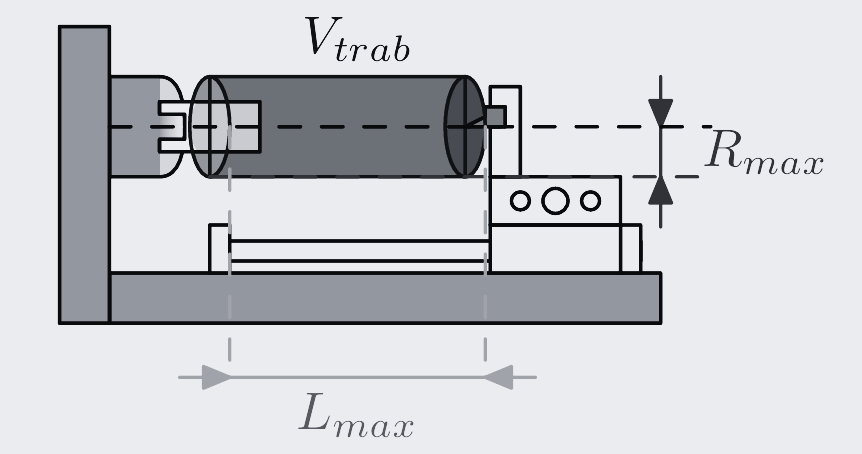
\includegraphics[width=0.8\linewidth]{images/vtrab.png}
    \caption{Representação gráfica do cálculo de volume de trabalho. Fonte: Autor.}
    \label{fig:vtrab}
\end{figure}

$$V_{trab} =(\pi R^2 Max) \cdot L_{Max}$$

$$R_{Max} = 50[mm]$$

$$L_{Max} = \text{Distância entre furos - Comprimento da mesa - Tamanho de um apoio}$$

$$L_{Max} =430[mm] - 130[mm] - 20[mm]$$

$$L_{Max} = 280[mm]$$

$$V_{trab} =(\pi \cdot 502) \cdot 280 = 2.199.114,86[mm^3]$$

$$V_{trab} = 0,0022[m^3]$$

\subsection{Velocidades dos Eixos}

O motor de passo KTC-HT23-400 apresenta uma relação inversa entre torque e velocidade, ou seja, à medida que o torque aumenta, a velocidade de rotação diminui. Quando se exige mais torque, a inércia do sistema também precisa ser minimizada para evitar perdas de eficiência e garantir que o motor funcione de maneira adequada.

A seguir, apresenta-se uma tabela que correlaciona os valores de velocidade e torque em função da massa móvel. Essa tabela fornece uma visão clara de como diferentes massas e torques impactam a velocidade e, consequentemente, a aceleração do sistema. A partir desses dados, será possível determinar os coeficientes de aceleração ideais para cada situação, garantindo que o motor funcione de forma eficiente e segura.

Para a obtenção da tabela, usaram as seguintes fórmulas: 
\begin{equation}
    J_{massa} = (m_{mesa} + m_{peca}) \cdot (\frac{p}{2\pi})^2
\end{equation}, para o cálculo do momento de inércia da carga. 

\begin{equation}
    J_{fuso} = \frac{1}{2} \cdot m_{fuso} \cdot (\frac{d_{fuso}}{2})^2
\end{equation}, para o cálculo do momento de inércia do fuso. 

Baseado na curva de torque da Seção 4.1, percebe-se que a velocidade do motor estará bem próxima da máxima, ou seja, 40[rev/s] e como o passo é 5[mm] temos que a velocidade dos eixos x e z em m/s é 0.2[m/s]. A velocidade média é de 0.1[m/s].  

Para estimar o momento de inércia do motor a partir da curva de torque versus velocidade, usou-se a relação entre o torque e a aceleração angular, dada pela equação:

\begin{equation}
    T = J \cdot \dot{\omega}
\end{equation}

Onde:
\begin{itemize}
    \item \( T \) é o torque (Nm),
    \item \( J \) é o momento de inércia (em kg $\cdot m^2$),
    \item \( \dot{\omega} \) é a aceleração angular (em $\frac{rad}{s^2}$).
\end{itemize}

A partir da curva, podemos identificar que o torque máximo \( T \) no modo Full Step é aproximadamente \( 1.4 \, \text{Nm} \), e a velocidade máxima do motor é \( 40 \, \text{rev/s} \). Para converter a velocidade em \( \text{rad/s} \), usamos a seguinte fórmula:

\begin{equation}
    \omega = 2\pi \cdot 40 \ = 251.2 \, \text{rad/s}
\end{equation}

Supondo que o motor acelere de \( 0 \, \text{rad/s} \) até \( 251.2 \, \text{rad/s} \) em \( 2 \, \text{segundos} \). A aceleração angular é então dada por:

\begin{equation}
    \dot{\omega} = \frac{\Delta \omega}{\Delta t} = \frac{251.2}{2} \, \text{rad/s²} = 125.6 \, \text{rad/s²}
\end{equation}

Substituindo os valores de \( T \) e \( \dot{\omega} \) na equação para o torque:

\begin{equation}
    1.4 = J \cdot 125.6
\end{equation}

Agora, resolvemos para \( J \):

\begin{equation}
    J = \frac{1.4}{125.6} = 0.01114 \, \text{kg} \cdot \text{m}^2
\end{equation}

Assim, o momento de inércia estimado do motor é aproximadamente:

\begin{equation}
    J_{motor} \approx 0.011 \, \text{kg} \cdot \text{m}^2
\end{equation}

A inércia acelerada será, portanto, 

\begin{equation}
    J_{carga} = J_{massa} + J_{fuso} + J_{motor} + J_{acoplamento} 
\end{equation}

Por fim, o torque de acionamento será obtido através da expressão:

\begin{equation}
    T_{acionamento} = J_{carga} \cdot \dot \omega + T_{atrito}
\end{equation}

Para o cálculo do torque de atrito, consideram-se aqueles gerados pelas guias lineareas, os mais de rolamento e os fusos. 

\begin{align}
    T_{guias} = \frac{p}{2\pi} \cdot \mu_{guias} \cdot [g(m_{mesa}+m_{peca})+F_{NormalCorte}] \\
    T_{mancal} = \mu \cdot \frac{d_{internoMancal}}{2} \cdot (F_{corte}+F_{préCarga}) \\
    T_{fuso} = \frac{p}{2\pi}\cdot F_{corte} \\
\end{align}

O torque de atrito final, portante, será dado pela expressão: 
\begin{equation}
    T = T_{guia} + T_{mancais} + T_{fuso}
\end{equation}

Por fim, chegou-se nos resultados da tabela abaixo. 

\begin{table}[h!] 
    \centering 
    \begin{tabular}{|c|c|c|} \hline 
        \textbf{Massa móvel [kg]} & \textbf{Torque [N.m]} & \textbf{Velocidade angular [rad/s]} \\ \hline 
        5 & 0,65 & 180 \\ \hline 
        8 & 0,80 & 160 \\ \hline 
        10 & 1,05 & 130 \\ \hline 
        12 & 1,25 & 110 \\ \hline 
    \end{tabular} 
    \caption{Correlação entre Massa Móvel, Torque e Velocidade Angular}  
\end{table}

A partir da análise da tabela, percebe-se que uma velocidade mais baixa requer um torque mais elevado, pois a resistência mecânica ou a carga aplicada ao motor aumenta. Nesses casos, o motor precisa aplicar mais força (torque) para continuar girando, o que pode comprometer a velocidade máxima atingível. Portanto, ao projetar a dinâmica do sistema, é essencial encontrar um equilíbrio entre torque, inércia e velocidade, ajustando os parâmetros de aceleração para que o motor atinja o torque necessário sem prejudicar a eficiência do sistema.

%%%%%%%%%%%%%%%%%%%%%%%%%%%%%%%%%%%%%%%%%%%%%%%%%%%%%%%%%%%%%%%%
\newpage
\section{Frequência Crítica do Laço Estrutural}

A frequência máxima de operação é de 30 Hz, limitada pelos motores utilizados, garantindo que a máquina opere abaixo de sua frequência natural para evitar ressonâncias.

%%%%%%%%%%%%%%%%%%%%%%%%%%%%%%%%%%%%%%%%%%%%%%%%%%%%%%5
\section{Tipo de sincronização entre os eixos}

Os movimentos dos eixos de uma máquina (como um torno ou fresadora) são coordenados para garantir que eles trabalhem em harmonia durante a operação. A sincronização é essencial para garantir a precisão nos processos de usinagem, já que o movimento de um eixo pode afetar diretamente o movimento do outro, especialmente em operações que requerem alta precisão.

A sincronização entre os eixos será feita por meio de uma \textbf{correia sincronizadora}. Ela é responsável por transmitir o movimento de forma simultânea entre os eixos, mantendo uma relação de velocidade constante. 

No presente projeto, a correia Optibelt ZR 345L cumpre essa função ao garantir que o movimento de um eixo seja replicado em outro de forma precisa, sem escorregamento, já que as correias sincronizadoras possuem dentes que se encaixam perfeitamente nas polias, evitando desvios.

Dentre as vantagens de utilizar esse tipo de sincronização entre eixos, é que esse é silencioso, requer pouca manutenção e oferece bom desempenho em termos de durabilidade e precisão.

%%%%%%%%%%%%%%%%%%%%%%%%%%%%%%%%%%%%%%%%%%%%%%%%%%%%%%%%%%%%%%%%

\section{Parâmetros de usinagem}

\subsection{Velocidade de corte}

A velocidade de corte refere-se à distância que a ferramenta percorre ao cortar o material em um determinado período de tempo. Esse parâmetro é crucial na operação de usinagem em um torno, pois permite calcular a rotação, em RPM, da placa de castanha, responsável por gerar a velocidade de corte no material. A velocidade de corte é determinada pela seguinte fórmula:

\begin{equation}
n=\frac{V_{C} \cdot 1000}{\pi d}    
\end{equation}

Onde: \\
- n  = rotação da máquina, em RPM; \\
- $\V_{C}$ = velocidade de corte, em m/min; \\
- d = diâmetro da peça, em mm. \\

Embora existam fórmulas para calcular a velocidade de corte, ela é frequentemente obtida em tabelas que já relacionam a operação, o material a ser usinado e o tipo de ferramenta de corte utilizada.

\begin{figure}[h!]
    \centering
    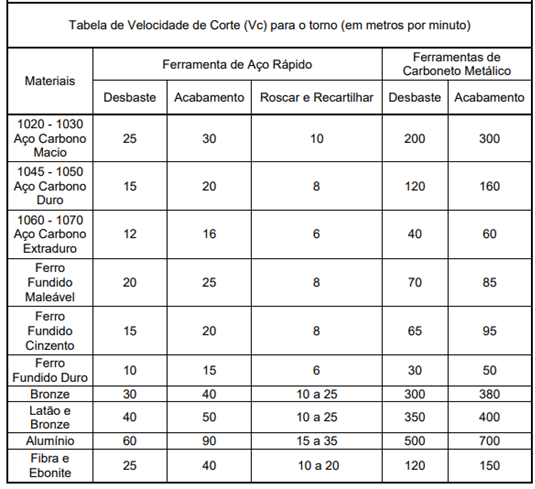
\includegraphics[width=0.7\linewidth]{images/vc_torno.png}
    \caption{Tabela de velocidade de corte para o torno (m/min).}
    \label{fig:enter-label}
\end{figure}

O Nylon 6.0 não está especificado na tabela acima, portanto, realizou-se uma pesquisa em sites de fabricantes de Nylon 6.0. De acordo com essas fontes, a velocidade de corte recomendada para o material varia entre 50 e 500 m/min, dependendo da operação realizada. Para o desbaste, utilizaremos uma velocidade de corte de 300 m/min. Com base nesse valor, é possível calcular a rotação necessária para usinar três tarugos de diferentes diâmetros: 25 mm, 50 mm e 100 mm.

Abaixo estão os cálculos da rotação necessária para manter a velocidade de corte de 300 m/min em cada um dos casos \cite{nylon6datasheet}:

Para 25mm de diâmetro:

\begin{align}
n=\frac{V_{C} \cdot 1000}{\pi d} = \frac{300 \cdot 1000}{\pi \cdot 25} = 3822 \text{rpm}
\end{align}

Para 50mm de diâmetro:

\begin{align}
n=\frac{V_{C} \cdot 1000}{\pi d} = \frac{300 \cdot 1000}{\pi \cdot 50} = 1911 \text{rpm}  
\end{align}

Para 100mm de diâmetro:

\begin{align}
n=\frac{V_{C} \cdot 1000}{\pi d} = \frac{300 \cdot 1000}{\pi \cdot 100} = 955 \text{rpm}
\end{align}

Esses valores são fundamentais, pois a utilização de velocidades de corte inadequadas na usinagem pode gerar diversos problemas. Quando a velocidade de corte está acima da recomendada, pode ocorrer o superaquecimento tanto da peça quanto da ferramenta, além da perda do fio de corte da ferramenta. Por outro lado, uma velocidade de corte abaixo do recomendado pode causar o travamento da ferramenta, muitas vezes resultando em sua quebra.

\subsection{Avanço de corte}

O avanço de corte representa a relação entre a velocidade de deslocamento da ferramenta e a velocidade da peça por rotação do eixo da máquina (mm/rotação). Ele depende diretamente da escolha da velocidade de corte, e, após essa definição, é necessário selecionar o avanço de corte adequado.
Assim como a velocidade de corte, o avanço de corte é fornecido por meio de tabelas disponibilizadas pelos fabricantes de ferramentas. Essas tabelas relacionam o material a ser usinado, o material da ferramenta e o tipo de operação a ser realizada. Abaixo está um exemplo de tabela de avanços de corte:

\begin{figure}[h!]
    \centering
    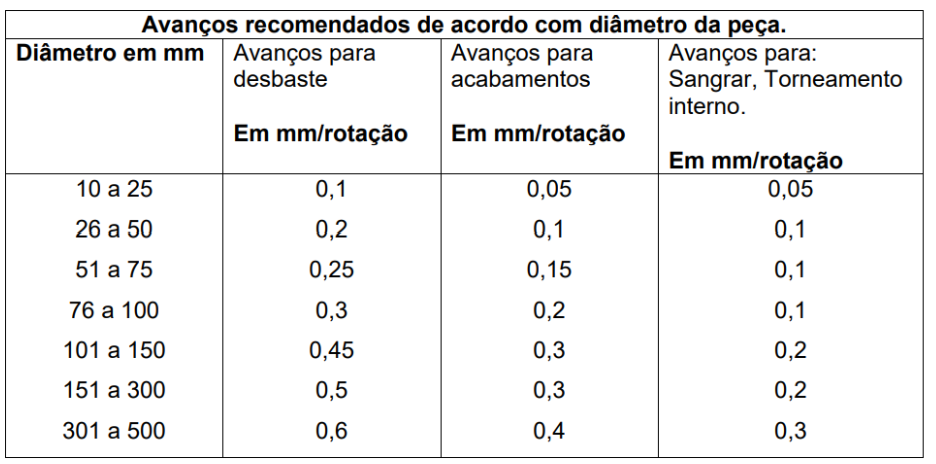
\includegraphics[width=0.7\linewidth]{images/avanco.png}
    \caption{Avaços recomendados de acordo com o diâmetro da peça.}
    \label{fig:enter-label}
\end{figure}

Para o caso do Nylon 6.0, os fabricantes recomendam um avanço de corte de 0,5 mm/rotação para operações de desbaste e 0,05 mm/rotação para operações de acabamento. Essas recomendações visam otimizar a qualidade do corte e a durabilidade da ferramenta, garantindo um bom equilíbrio entre eficiência e precisão durante o processo de usinagem.